\subsection{Hauptprogramm State Machine}\label{subsec:State_Machine}
Abbildung \ref{img:state_machine} zeigt links die Initialisierung und rechts den Hauptprogrammfluss der Software als State Machine.
\begin{figure}[h]
	\centering
	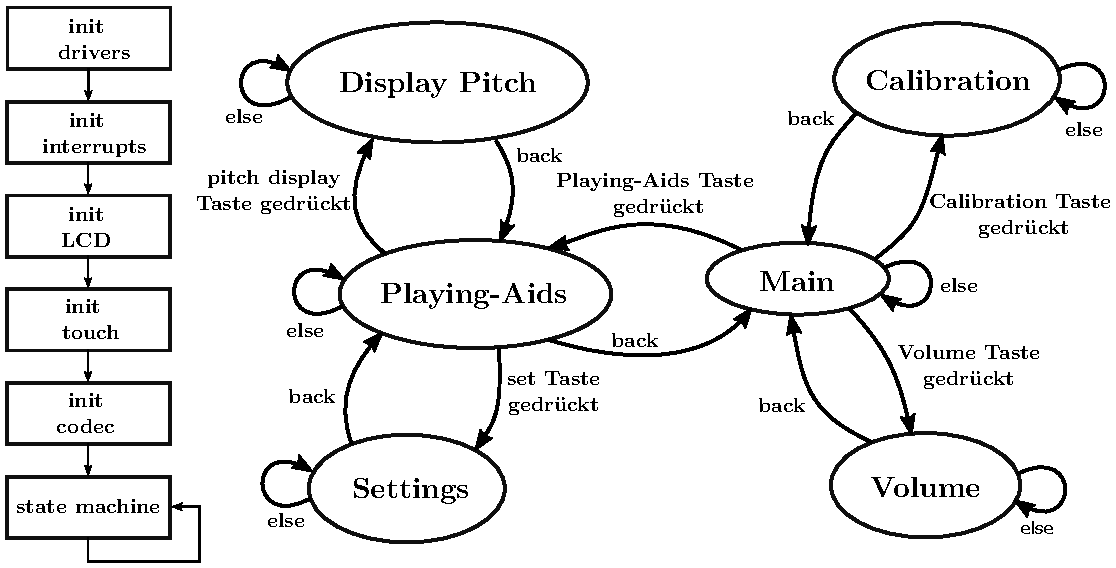
\includegraphics[width=\textwidth]{state_machine.pdf}
	\caption{State Machine und Initailisierung.}
	\label{img:state_machine}
\end{figure}

Als erstes initialisiert das Programm alle Treiber, den Touchscreen, das LCD, und den Codec. Anschliessend führt das Programm in einer Endlosschlaufe die State Machine aus. Es folgen kurze Erklärungen zu jedem State.

\textbf{Main}:
Dies ist der erste State nachdem Initialisierungsvorgang. Der Main State wartet auf eine Betätigung der drei in Abbildung \ref{img:main_screen} gezeigten Tastern. Eine Betätigung der drei Tastern führt zu einem Wechsel in den entsprechenden State. 
 
\textbf{Calibration}:
Der Calibration State fordert den Benutzer auf seine rechte Hand in die Nähe der rechten Antenne zu halten.
Nach zwei Sekunden startet die Kalibrierung. Sobald die Kalibrierung abgeschlossen ist, kann der Benutzer über den \textit{back} Taster zurück in den Main State gelangen. Abbildung \ref{img:calibration_screen} zeigt die Darstellung des LCD nach erfolgreicher Kalibrierung.

\textbf{Volume}:
In diesem State kann der Benutzer die Lautstärke ändern und die Lautstärkenantenne aktivieren und deaktivieren. Die Lautstärke kann in 10 verschiedene Pegeln eingestellt werden. Dies geschieht mithilfe der in Abbildung \ref{img:vol_screen} gezeigten \textbf{\textit{+}} und \textbf{\textit{-}} Tasten. Beim betätigen der \textit{vol antenna} Taste wird die Lautstärkenantenne je nach aktuellem Zustand deaktiviert oder aktiviert. Mit dem betätigen der \textit{back} Taste gelangt der Benutzer in den Main State.
 
\textbf{Playing-Aids}:
Im State Playing Aids kann der Benutzer mit der\textit{Glissando on} Taste den Glissando-Effekt aktivieren und deaktivieren. Die Abbildungen \ref{img:play_aids_off} und \ref{img:play_aids_on} zeigen die grafische Realisierung dieser Taste. Über die \textit{Set} Taste gelangt der Benutzer in den State Settings. Durch betätigen des \textit{display pitch} Taste wird in den State Pitch Display gewechselt. Zurück in den Main State gelangt man über die \textit{back} Taste.

\textbf{Settings}:
Im Settings State können Einstellungen am Glissando-Effekt gemacht werden. Der Delay des Glissando-Effekts ist in 10 Stufen einstellbar. Zudem kann der Anwender mit dem Taster \textit{pentatonic on/off} zwischen der pentatonischen und der normalen Tonleiter wechseln. Mit dem betätigen der \textit{back} Taste gelangt der Benutzer in den Playing-Aids State. Abbildung \ref{img:settings_screen} zeigt wie der Setting State auf dem LCD aussieht.

\textbf{Pitch Display}:
Dieser State unterstützt den Theremin Spieler dabei Töne der Tonleiter zu treffen. Der Spieler bekommt über das Display eine optische Rückmeldung in welcher Region der Tonleiter sich der gespielte Ton befindet. So muss der Spieler nicht alleine auf sein Gehör vertrauen.
Abbildung \ref{img:play_help_screen} zeigt die Darstellung dieses States.  
Der Schriftzug oberhalb des LCD zeigt den Ton an, der sich in der Region der gespielten Frequenz befindet. 
Der kleine vertikale Strich zeigt dem Spieler an wie weit weg die aktuell gespielte Frequenz von dem Ton der Tonleiter ist. 
Diese graphische Unterstützung kann jedoch nur bei der pentatonischen Tonleiter angewendet werden. Da die Antenne sehr empfindlich auf Änderungen ist, ist es mit der normalen Tonleiter nicht hilfreich den vertikalen Strich anzuzeigen. Daher haben wir uns entschieden diese Anzeige nur bei der pentatonischen Tonleiter zu verwenden.

\begin{figure}[!ht]
	\subfloat[Main Menu\label{img:main_screen}]{%
		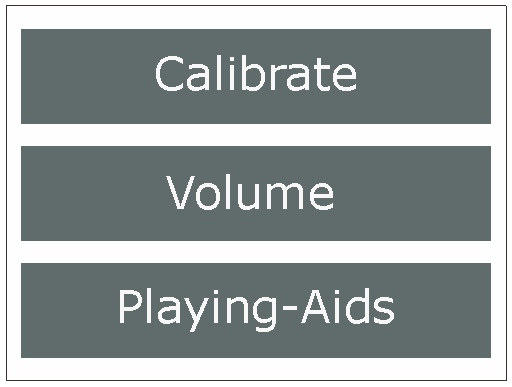
\includegraphics[width=0.3\textwidth]{Main.pdf}
	}
	\hfill
	\subfloat[Calibration Menu\label{img:calibration_screen}]{%
		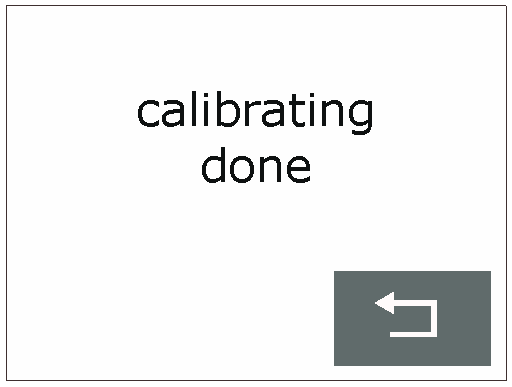
\includegraphics[width=0.3\textwidth]{calibrating_done.pdf}
	}
	\hfill
	\subfloat[Volume Menu\label{img:vol_screen}]{%
		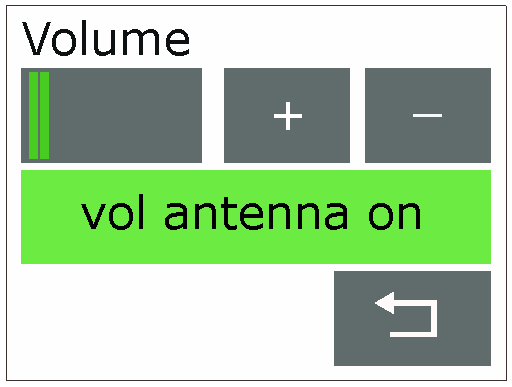
\includegraphics[width=0.3\textwidth]{volume.pdf}
	}
	\\
	\subfloat[Playing-Aids Menu, Glissando off\label{img:play_aids_off}]{%
		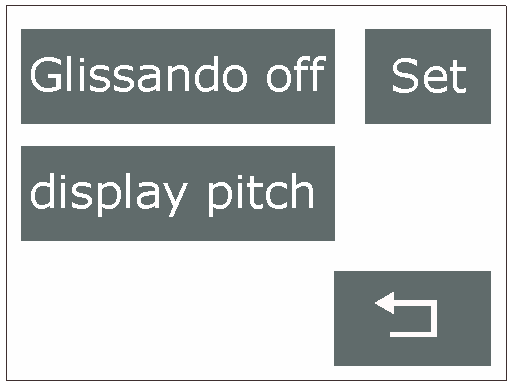
\includegraphics[width=0.3\textwidth]{play_aids.pdf}
	}
	\hfill
	\subfloat[Playing-Aids Menu, Glissando on\label{img:play_aids_on}]{%
		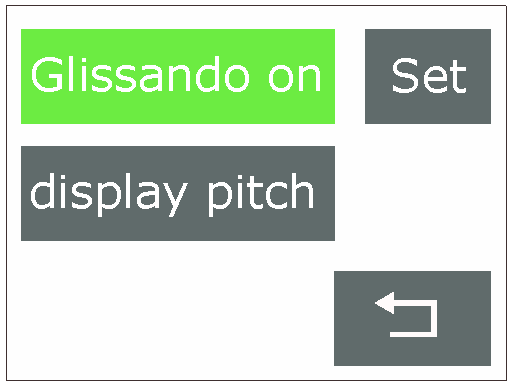
\includegraphics[width=0.3\textwidth]{play_aids_on.pdf}
	}
	\hfill
	\subfloat[Settings Menu\label{img:settings_screen}]{%
		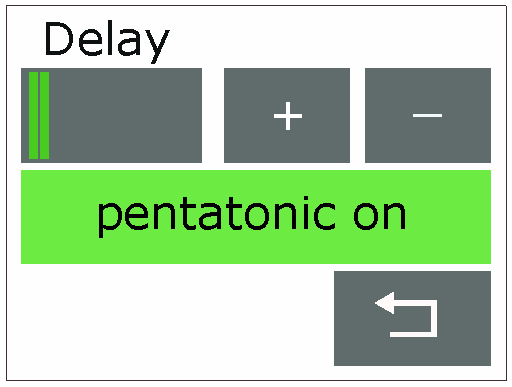
\includegraphics[width=0.3\textwidth]{settings.pdf}
	}
	\\
	\subfloat[Play help Menu\label{img:play_help_screen}]{%
		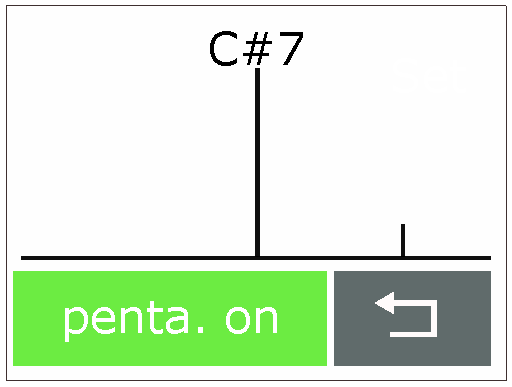
\includegraphics[width=0.3\textwidth]{pitch_display.pdf}
	}
	\hfill

	\caption{Dummy figure}
	\label{fig:dummy}
\end{figure}
